\documentclass[10pt]{article}
\usepackage[UTF8]{ctex}
\usepackage{picinpar,graphicx,bm}
\usepackage{booktabs}
\usepackage{diagbox}
\usepackage{float}
\usepackage{setspace}

% used to demo bracket for array
\usepackage{amsmath}

\usepackage{listings}
\usepackage{xcolor}
% 定义可能使用到的颜色
\definecolor{CPPLight}  {HTML} {686868}
\definecolor{CPPSteel}  {HTML} {888888}
\definecolor{CPPDark}   {HTML} {262626}
\definecolor{CPPBlue}   {HTML} {4172A3}
\definecolor{CPPGreen}  {HTML} {487818}
\definecolor{CPPBrown}  {HTML} {A07040}
\definecolor{CPPRed}    {HTML} {AD4D3A}
\definecolor{CPPViolet} {HTML} {7040A0}
\definecolor{CPPGray}  {HTML} {B8B8B8}
\lstset{
    columns=fixed,    
   % numbers=left,                                        % 在左侧显示行号
    frame=none,                                          % 不显示背景边框
    backgroundcolor=\color[RGB]{245,245,244},            % 设定背景颜色
    keywordstyle=\color[RGB]{40,40,255},                 % 设定关键字颜色
    numberstyle=\footnotesize\color{darkgray},           % 设定行号格式
    commentstyle=\it\color[RGB]{0,96,96},                % 设置代码注释的格式
    stringstyle=\rmfamily\slshape\color[RGB]{128,0,0},   % 设置字符串格式
    showstringspaces=false,                              % 不显示字符串中的空格
    language=c++,                                        % 设置语言
    morekeywords={alignas,continute,friend,register,true,alignof,decltype,goto,
    reinterpret_cast,try,asm,defult,if,return,typedef,auto,delete,inline,short,
    typeid,bool,do,int,signed,typename,break,double,long,sizeof,union,case,
    dynamic_cast,mutable,static,unsigned,catch,else,namespace,static_assert,using,
    char,enum,new,static_cast,virtual,char16_t,char32_t,explict,noexcept,struct,
    void,export,nullptr,switch,volatile,class,extern,operator,template,wchar_t,
    const,false,private,this,while,constexpr,float,protected,thread_local,
    const_cast,for,public,throw,std,size_t,__global__,__device__,__host__},
    emph={map,set,multimap,multiset,unordered_map,unordered_set,
    unordered_multiset,unordered_multimap,vector,string,list,deque,
    array,stack,forwared_list,iostream,memory,shared_ptr,unique_ptr,
    random,bitset,ostream,istream,cout,cin,endl,move,default_random_engine,
    uniform_int_distribution,iterator,algorithm,functional,bing,numeric,},
    emphstyle=\color{CPPViolet}, 
    frame=shadowbox,
    basicstyle=\footnotesize\ttfamily,
    tabsize=4,
}


%layout
\usepackage{calc} 
\setlength\textwidth{7in} 
\setlength\textheight{9in} 
\setlength\oddsidemargin{(\paperwidth-\textwidth)/2 - 1in}
\setlength\topmargin{(\paperheight-\textheight -\headheight-\headsep-\footskip)/2 - 1.5in}


\title{应用几何造型 \hspace{2pt}\hspace{2pt} \begin{large}----- \hspace{2pt} B-spline曲面拟合 \end{large} }
\author{11821095 葛林林}
\begin{document}
\maketitle


\section{预备知识}
\subsection{B-spline曲线的表示}
\paragraph{B-spline基函数:}
定义$B_{k,m}(t)$为B-spline基函数如下所示
$$
\left\{
\begin{array}{rl}
B_{k,m}(t)&:=\displaystyle\frac{t-t_k}{t_{k+m-1}-t_k}B_{k,m-1}(t)+\frac{t_{k+m}-t}{t_{k+m}-t_{k+1}}B_{k+1,m-1}(t)\\
B_{k,1}(t)&:=
\left\{
\begin{array}{l}
1 \hspace{10pt} t_k \leq t < t_{k+1} \\
0 \hspace{10pt} other
\end{array}
\right.\\
asume \hspace{5pt} \frac{0}{0}&:=0
\end{array}
\right. 
$$
其中,$k$代表第$k$个基函数,$m-1$为该基函数的次数。
\paragraph{B-spline的定义:}在基函数的基础上,定义B-spline曲线方程如下所示
$$P(t):=\sum_{i=0}^{N}\bm{P}_iB_{i,m}(t)$$
其中,$\bm{P}_i$代表了控制顶点,用点坐标表示,总共有$N+1$个控制顶点,每个B-spline基函数为$m-1$次。而$t$为节点,所有的节点组成了节点向量$\bm{T}=[t_{0},t_1,t_2,\cdots,t_{N+m}]^T$。

\subsection{B-spline曲线的拟合}
\paragraph{目标函数}\mbox{}\\
假设$D_i$为已知的数据集合,则目标函数可以可以表示如下:
$$E(t):=\sum_{k=0}^{K}|D_k-P(t_k)|^2=\sum_{k=0}^K|D_i-\sum_{i=0}^N\bm{P}_iB_{i,m}(t_k)|^2$$
令
$$\bm{D}=\left[D_1 \hspace{10pt} D_2 \hspace{10pt} \cdots \hspace{10pt} D_N\right] ^T$$
$$\bm{N}=
\left[
\begin{array}{cccc}
B_{1,1}(t_1) \hspace{10pt} B_{1,1}(t_2) \hspace{10pt} \cdots \hspace{10pt} B_{1,1}(t_K) \\
B_{2,1}(t_1) \hspace{10pt} B_{2,1}(t_2) \hspace{10pt} \cdots \hspace{10pt} B_{2,1}(t_K)\\
\cdots \hspace{10pt} \cdots \hspace{10pt} \cdots \hspace{10pt} \cdots \\
B_{N,1}(t_1) \hspace{10pt} B_{N,1}(t_2) \hspace{10pt} \cdots \hspace{10pt} B_{N,1}(t_K)
\end{array}
\right]
$$

$$\bm{P}=
\left[
\bm{P}_1 \hspace{10pt} \bm{P}_2 \hspace{10pt} \cdots \hspace{10pt} \bm{P}_N
\right]^T
$$
则目标函数可以转化为如下公式:
$$\bm{E}=(\bm{D}-\bm{N}^T\bm{P})^T(\bm{D}-\bm{N}^T\bm{P})$$
$$\frac{\partial{\bm{E}}}{\partial{\bm{P}}}=2(-\bm{N}^T)(\bm{D}-\bm{N}^T\bm{P})=0$$
则有
$$\bm{D}-\bm{N}^T\bm{P}=0$$
既
$$\bm{D}=\bm{N}^T\bm{P}$$
则可以得到控制点$\bm{P}$为:
$$\bm{P}=(\bm{N}^T\bm{N})^{-1}\bm{N}^T\bm{D}$$
\subsection{B-spline曲面的表示}
\paragraph{B-spline曲面的定义:}
$$P(u,v):=\sum_{i=0}^{M}\sum_{j=0}^{N}\bm{P}_{i,j}B_{i,m}(u)B_{j,n}(v)$$
其中$B_{i,m}(u),B_{j,n}(v)$为B-spline基函数,$\bm{P}_{i,j}$代表控制顶点。

\subsection{曲面的拟合}
\paragraph{目标函数}\mbox{} \\
假设$D_{a,b}$是曲面上的数据点,定义误差函数如下所示:
$$
E(\bm{P}_{00},\bm{P}_{01},\cdots,\bm{P}_{MN}):=\displaystyle\sum_{a=0}^A\sum_{b=0}^B|D_{a,b}-P(u_a,v_b)|^2=\displaystyle\sum_{a=0}^A\sum_{b=0}^B|D_{a,b}-\sum_{i=0}^{M}\sum_{j=0}^{N}\bm{P}_{i,j}B_{i,m}(u_a)B_{j,n}(v_b)|^2
$$

\paragraph{推导}\mbox{} \\
对目标函数求偏导可以得到如下公式:
$$
\displaystyle\frac{\partial{E}}{\partial{\bm{P}_{cd}}}=\displaystyle\sum_{a=0}^{A}\sum_{b=0}^B
\left[
2\left(
D_{a,b}-\sum_{i=0}^M\sum_{j=0}^N\bm{P}_{ij}B_{i,m}(u_a)B_{j,n}(v_b)
\right)
\left(
-\sum_{c=0}^M\sum_{d=0}^NB_{c,m}(u_a)B_{d,n}(v_b)
\right)
\right]=0
$$
通过该公式很难得到解析解,因此可以借助曲线拟合的结果对曲面得到一个近似的结果其算法思路如下
\begin{figure}[H]
\begin{center}
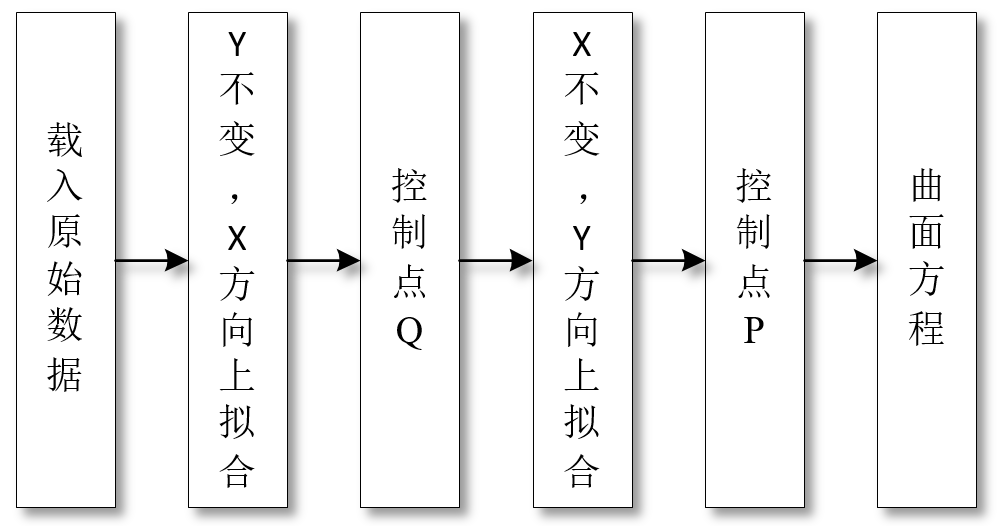
\includegraphics[scale=0.4]{algorithm1.png}
\caption{算法步骤}
\end{center}
\end{figure}

\section{实验结果}
本报告中实验所使用的开发环境如下所示:
\begin{table}[H]
\caption{环境参数}
\begin{center}
\begin{tabular}{ll}
\toprule  %添加表格头部粗线
参数& 描述\\
\midrule  %添加表格中横线
System& Windows 10 64bit \\
CPU& Intel(R) Core(TM) i5-2410M CPU @2.30GHz 2.3GHz(4核)\\
RAM& 6GB\\
IDE& Visual Studio 2017 \\
Library& Eigen, OpenGL\\
\bottomrule %添加表格底部粗线
\end{tabular}
\end{center}
\end{table}

如下所示是得到的原始图和结果图对比:
\begin{figure}[H]
\begin{center}
\begin{minipage}[t]{0.45\linewidth}
\centering
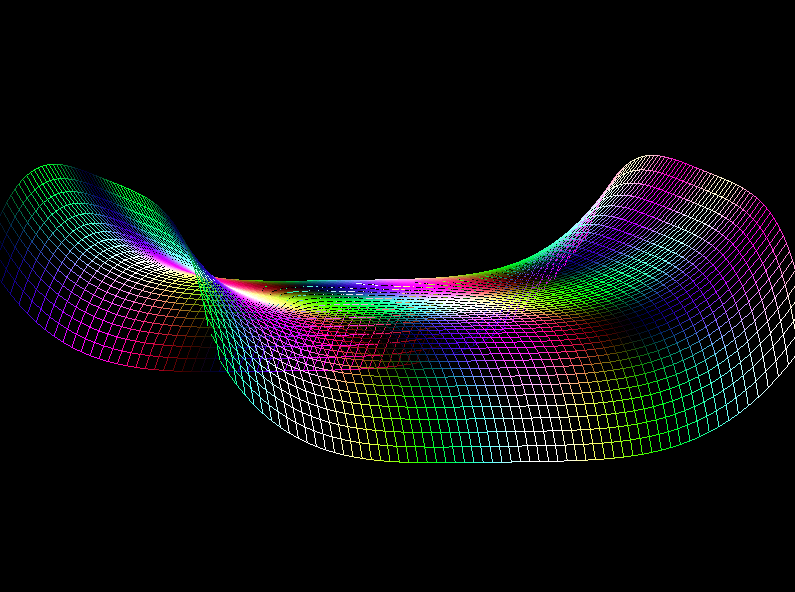
\includegraphics[scale=0.35]{saddle_raw.png}
\caption{原始曲面}
\end{minipage}%
\begin{minipage}[t]{0.45\linewidth}
\centering
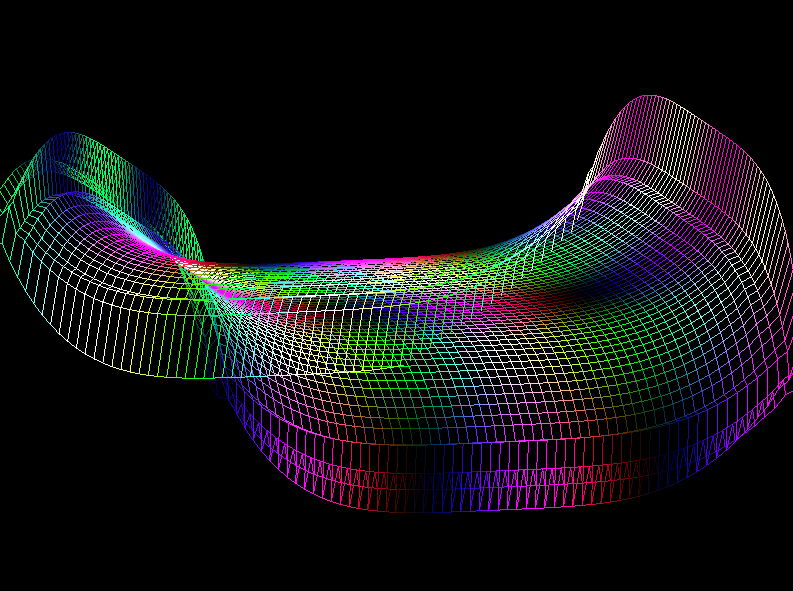
\includegraphics[scale=0.35]{saddle_out.png}
\caption{拟合曲面}
\end{minipage}
\end{center}
\end{figure}

\begin{figure}[H]
\begin{center}
\begin{minipage}[t]{0.45\linewidth}
\centering
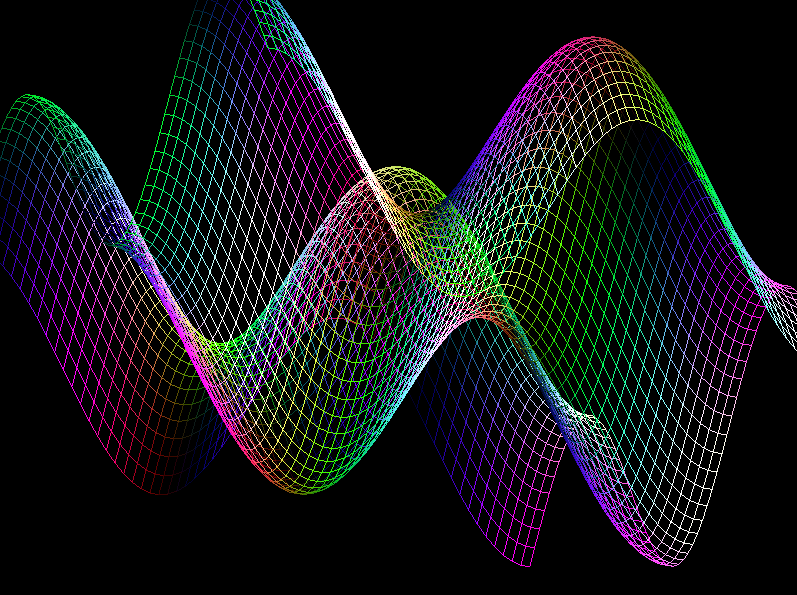
\includegraphics[scale=0.35]{shape2_raw.png}
\caption{原始曲面}
\end{minipage}%
\begin{minipage}[t]{0.45\linewidth}
\centering
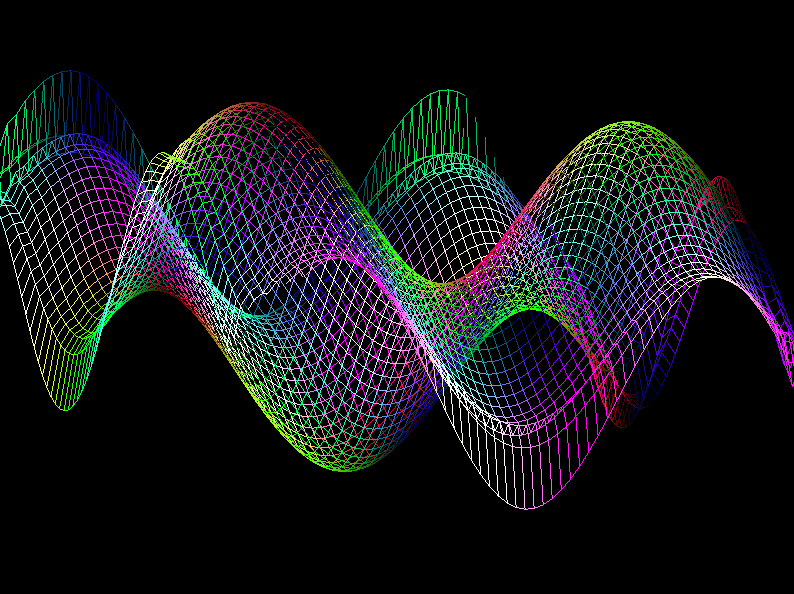
\includegraphics[scale=0.35]{shape2_out.png}
\caption{拟合曲面}
\end{minipage}
\end{center}
\end{figure}

\section{问题汇总}
\subsection{控制节点和节点向量的个数如何选取?} 
控制节点和节点向量个数之间存在关系,假设控制节点个数为$M$,节点向量个数为$N$,b样条的次数为$m$,则满足如下关系:
$$M=N+m+1$$
因此一旦确定了节点向量的个数和b样条的次数就可以确定控制节点的个数。而节点向量的个数可以根据需要拟合的数据范围进行调整,范围越大节点向量的个数越多。

\subsection{控制顶点与基函数相乘如何运算?}
控制顶点可以看做一个向量,因此曲线或者曲面上的$x$和$y$轴坐标都需要根据定义计算出来。假设$P_i=[x_i         \hspace{5pt} y_i]^T$,则B-spline曲线可以表示为如下形式:
$$P(t):=\sum_{i=0}^{N}
\left(
\begin{array}{c}
x_i \\
y_i
\end{array}
\right)
B_{i,m}(t)
$$

\end{document}